\Chapter{Tervezés}
Ez a fejezet a program tervezésével kapcsolatos információkat, specifikációkat tartalmazza. Egy látványterv leírása a felhasználói felületről és a szükséges funkciókról.

\Section{Grafikus Felhasználói Felület (GUI) - megjelenés, funkció}

Az alkalmazás két menüpontből álljon, jegyzetek és kereső menü. A két menü működése egyedi objektumok használatával történjen.

\subsection{Szükséges adattípusok}
Szükséges egy Note és egy Page objektum konstruktor létrehozása.
\\A Note objektumnak legyenek a következő változói:
\begin{itemize}
	\item String noteName - A jegyzet neve.
	\item ArrayList<Page> pageList - Egy Page típusú ArrayList a jegyzet oldalainak tárolására. Egyszerűen lehet majd törölni és hozzáadni új Page objektumokat.
	\item int Id - Egy ID az egyszerű azonosítás érdekében.
	\item static int counter - Egy számláló, ami majd az ID-t növeli, maga a számláló értékét pedig a konstruktorban kell növelni.
	\item Minden adathoz a megfelelő getter-setter metódusok.
\end{itemize}

\vspace{10pt} \noindent A Page objektumnak legyenek a következő változói:
\begin{itemize}
	\item String pageName - Az oldal neve.
	\item String pageText - Az oldal tartalma, a szövegdobozba írt adatok.
	\item int noteId - A lapot tartalmazó jegyzet ID-je ahhoz, hogy egyszerűen meghatározható legyen a kapcsolat egy Note és egy Page objektum között.
	\item int Id - Egy ID az egyszerű azonosítás érdekében.
	\item static int counter - Egy számláló, ami majd az ID-t növeli, maga a számláló értékét pedig a konstruktorban kell növelni.
	\item Minden adathoz a megfelelő getter-setter metódusok.
\end{itemize}

\subsection{Közös elemek}

A következő elemek olyanok, amelyeknek mindkét menüpontban látszaniuk kell és használhatóak kell legyenek. A \ref{fig:main_foundation}. ábrán pirossal bekeretezett és számozott részek ezeket az elemeket jelzik, leírásuk számozva, a kép alatt található.

\begin{figure}[h]
	\centering
	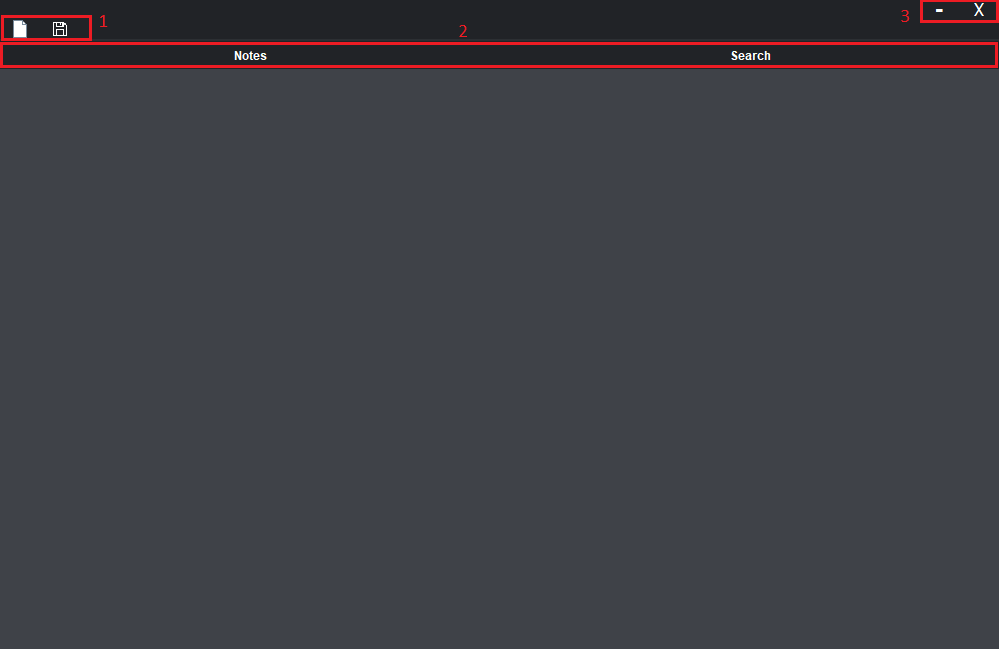
\includegraphics[scale=0.5]{images/menu_1.png}
	\caption{Program 'körvonala', alapja, a felület amire a többi menü épül.}
	\label{fig:main_foundation}
\end{figure}

\noindent \textbf{1.} Gombok helye. Fájl megnyitása és mentése gombra gondoltam. Ha további gombok hozzáadása szükséges lenne,  azok is ide kerülnének, feltéve ha mindegyik menüpontban használhatóak.
\vspace{5pt} \\Fájl megnyitása gomb (4.1 ábrán az 1.ikon): lokális adatbázis használata esetén lehet fontos. Szükségessége attól függ, hogy lokális vagy felhőalapú adatbázis kerül felhasználásra.
\vspace{5pt} \\Fájl mentése gomb (4.1 ábrán a 2. ikon): elmenti az adatok változásait, amiket a későbbiekben az adatbázisba kell töltsön.
\vspace{5pt} \\ \textbf{2.} Két menüpont váltására alkalmas gombok helye, ezekre kattintva válthatunk a menük között.
\vspace{5pt} \\ \textbf{3.} Bezár és tálcáz gombok, funkcióik egyértelműeknek tartom.
\vspace{10pt} \\Az alkalmazás ablak bárhová legyen elhelyezhető a képernyőn (tehát lehessen húzgálni), amíg a felső sötétebb színű sávon tartjuk lenyomva  a bal egérgombot, viszont átméretezni ne lehessen.
\vspace{5pt} \\Belépéskor ez a kép fogadja a felhasználót, egyik menüpontban se legyen benne. 

\subsection{Jegyzetek menü}

A \ref{fig:menu_notes}. ábrán látható a jegyzetek menü elképzelt felépítése A pirossal számozott elemek leírása található a kép alatt, elmondja, hogy milyen funkciókat kell majd, hogy az egyes elemek betöltsenek.

\begin{figure}[h]
	\centering
	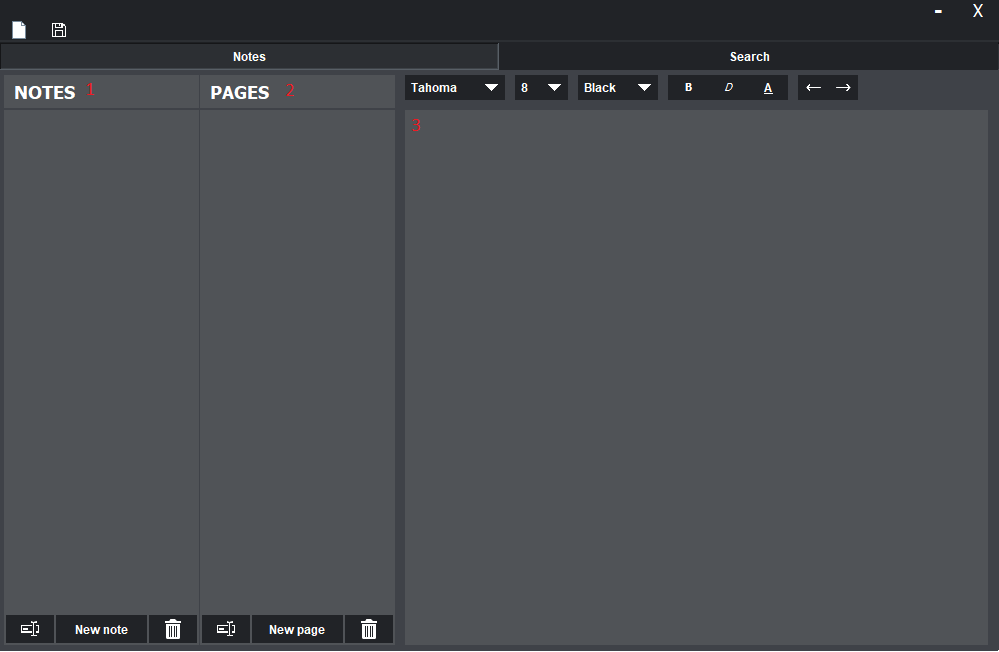
\includegraphics[scale=0.5]{images/menu_2.png}
	\caption{Jegyzetek menü}
	\label{fig:menu_notes}
\end{figure}

\vspace{5pt} \noindent \textbf{1.} Jegyzetek (Note objektumok) listája, ahol a jegyzetek neve jelenik meg egymás alatt. 
\\Ha betelne a jegyzetek listája, akkor a görgő segítségével lehet köztük navigálni.
\\Átnevezni, létrehozni és törölni jegyzeteket a lista alján található gombokkal lehessen. A gombok csak a kijelölt jegyzetet szerkesszék!
\vspace{5pt} \\ \textbf{2.} Oldalak (Page objektumok) listája. Ha nincs jegyzet kiválasztva, akkor a lista alapvetően üres legyen. Az éppen kijelölt (rákattintott) jegyzet oldalainak nevei legyenek itt felsorolva. 
\\Egy jegyzethez több oldal is létrehozható, de egy adott oldal csak egy meghatározott jegyzethez tartozhat (feltéve ha nem másoltuk be egy másik jegyzetbe ugyan azt a szöveget és adtunk a lapunknak hasonló címet). 
\\Ha betelne az oldalak listája, akkor a görgő segítségével lehessen köztük navigálni. 
\\Átnevezni, létrehozni és törölni oldalakat a lista alján található gombokkal lehetséges. A gombok csak a kijelölt oldalakat szerkesszék!
\\Ha nincs kijelölve jegyzet, akkor a lapok listája is legyen üres.
\vspace{5pt} \\ \textbf{3.} Szövegszerkesztő, az éppen kijelölt oldal tartalma legyen itt látható és szerkeszthető. 
\\Ha nincs oldal kijelölve, akkor ne legyen használható a szerkesztő és ne jelenjen meg benne szöveg. 
\vspace{5pt} \\Legyenek elérhetők szöveg szerkesztésére alkalmas gombok, amelyek funckiói a következők: 
\begin{itemize}
	\item Betűstílus, betűméret és szín megadására alkalmas legördülő választási menü.
	\item Szöveg dőltté, vastaggá és aláhúzottá alakító gombok. Ki-bekapcsolóként működjenek.
	\item Undo gomb, ami az előző szerkesztést vonja vissza.
	\item Redo gomb, ami az előzőleg visszavont szerkesztést csinálja újra.
\end{itemize}
Az első és második pontban leírt funkcióknak csak a kijelölt szövegen legyen hatása.
\\A gombok legyenek gyorsbillentyűkkel is használhatók.


\subsection{Kereső menü}

A \ref{fig:menu_search}. ábrán látható a kereső menü elképzelt felépítése A pirossal számozott elemek leírása található a kép alatt, elmondja, hogy milyen funkciókat kell majd, hogy az egyes elemek betöltsenek.

\begin{figure}[h]
	\centering
	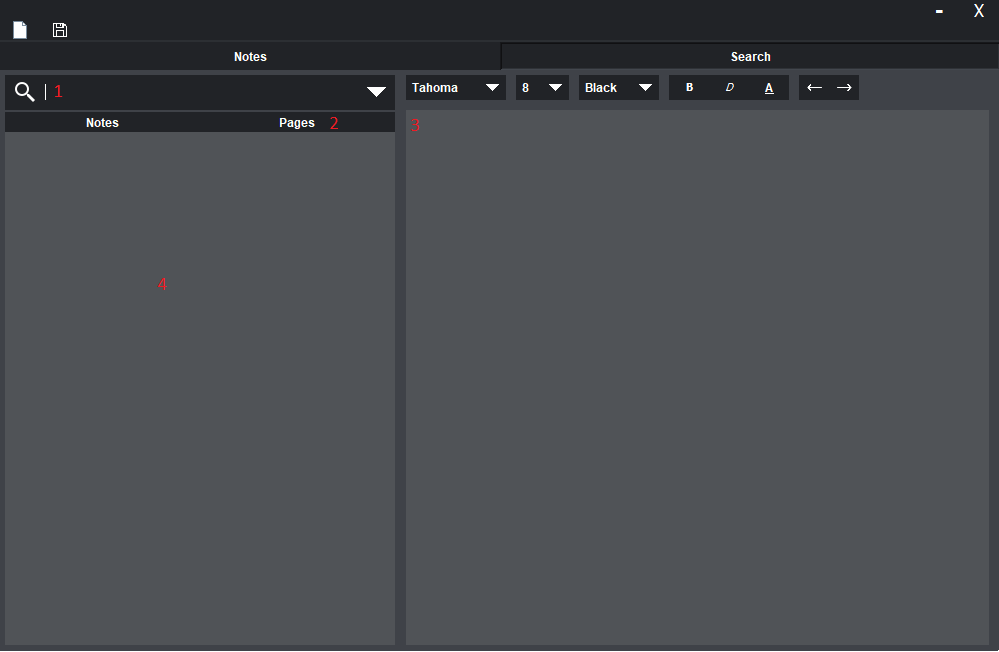
\includegraphics[scale=0.5]{images/menu_3.png}
	\caption{Kereső menü}
	\label{fig:menu_search}
\end{figure}

\vspace{5pt} \noindent \textbf{1.} Kereső sáv. Ne legyen case-sensitive, tehát ne tegyen kis- és nagybetű között különbséget.
\\Jegyzet- és oldalnevek, és az oldalak tartalma között is keressen egyező adatokat.
\\Jelenjen meg egy legördülő menü ahogy írjuk a szöveget, ami a találatok nevét tartalmazza. Tehát ha egyezést talál a beírt szöveg és 
\begin{itemize}
	\item egy jegyzet neve között, akkor a jegyzet neve jelenjen meg.
	\item egy lap neve között, akkor a lap neve jelenjen meg.
	\item egy lap tartalma között, akkor a tartalmazó lap neve jelenjen meg.
\end{itemize}
Beírt szövegre a nagyító gombra való kattintással tudjunk keresni, vagy a legördülő menüben megjelenő találatokra kattintva. 
\vspace{5pt} \\ \textbf{2.} Talált jegyzetek és lapok között a két adott gombbal lehessen váltani. Jelenjen meg a kiválasztott találatok listája.
\\Gombra való kattintással lehessen kiválasztani hogy melyik lista látszódjon.
\vspace{5pt} \\ \textbf{3.} A jegyzetek menünél bemutatott szövegszerkesztő, melynek működése legyen megegyező.
A kijelölt lap szövege jelenjen meg itt, legyen szerkeszthető.
\vspace{5pt} \\ \textbf{4.} A 2. pontban jellemzett gombok esetén két lehetőség legyen: vagy a jegyzetek listája látszódjon, vagy a lapok listája. 
\\A listák az érvényes találatokat tartalmazzák.
\\Lehessen a listák elemei között (úgy mint a jegyzetek menüben) kattintással választani. Ilyenkor további két lehetőség legyen:
\begin{itemize}
	\item Ha egy jegyzet listaelemet választunk, akkor a program tegyen át a jegyzetek menüpontba, és legyen a kiválasztott jegyzet kijelölve. Ha a jegyzetet görgetéssel lehet elérni, akkor a görgő is legyen a megfelelő pozícióba úgy, hogy látszódjon a listán a kiválasztott elem. Lapja ne legyen kijelölve, szövegdoboz legyen üres.
	\item Ha egy lap listaelemet választunk, akkor a szövegdobozban jelenjen meg a  tartalma. Legyen itt is szerkeszthető a tartalom.
\end{itemize}

\Section{Adatbázis}
Az adatok adatbázisba legyenek eltárolva, vagy felhőalapú adatbázisba, vagy lokális adatbázisba. 
\\Ha lokális adatbázisra esik a választás, az adatok szinkronizálása több eszköz között legyen megoldva.
\\Adatbázishoz való csatlakozás a programkódban legyen megfelelően implementálva.


\Section{Titkosítás}
A titkosítási algoritmus tesztek alapján a legjobbnak vélt algoritmussal kerüljenek az adatok kódolásra.
\\A titkosítás vagy alkalmazás szinten, saját implementációval legyen megoldva vagy a tárolástól függően az ismertetett adatbázis titkosítási módszerek egyikének alkalmazásával.
\\Mivel az alkalmazás minden esetben az adathalmaz egészével dolgozik, ezért elegendő lehet, ha egy xml vagy json fájl kerül titkosításra, amely az összes adatot tartalmazza, nem pedig minden adat egyesével.
\\A titkosítási kulcsok legyenek biztonságosan tárolva, több eszköz között biztonságosan megosztva.
\\Az alkalmazás bezárása előtt kerüljenek át az adatok az adatbázisba. Alkalmazás megnyitása után kerüljenek beolvasásra majd megjelenítésre.
